\section{Supplement}

This section contains algorithms, proofs, and experiments in support of the main text.

\subsection{Algorithms}
\label{sec:algorithms}

We give definitions of the brute and greedy algorithms for the combinatorial problem studied in this paper.
The brute force algorithm is computationally intractable for all but the smallest problems, but always finds the global minima.

\begin{algorithm}[H]
\caption{\brute(Matrix ${X} \in \mathbb{R}^{D \times P}$, objective $f$)}
\begin{algorithmic}[1]
\FOR{each combination $S \subseteq \{1, 2, \dots, P\}$ with $|S| = D$}
    \STATE Evaluate $f({X}_{.S})$
\ENDFOR
\STATE {\bf Output} the combination $S^*$ that minimizes $f({X}_{.S})$
\end{algorithmic}
\end{algorithm}

Greedy algorithms are computationally expedient but can get stuck in local optima \citep{Cormen, Russell-09}, even with randomized restarts \citep{Dick2014HowMR}.

\begin{algorithm}[H]
\caption{\greedy(Matrix ${X} \in \mathbb{R}^{D \times P}$, objective $f$, selected set $S = \emptyset$, current size $d=0$)}
\begin{algorithmic}[1]
\IF{$d = D$}
    \STATE {\bf Return} $S$
\ELSE
    \STATE {\bf Initialize} $S_{\text{best}} = S$
    \STATE {\bf Initialize} $f_{\text{best}} = \infty$
    \FOR{each $p \in \{1, 2, \dots, P\} \setminus S$}
        \STATE {\bf Evaluate} $f({X}_{.(S \cup \{p\})})$
        \IF{$f({X}_{.(S \cup \{p\})}) < f_{\text{best}}$}
            \STATE {\bf Update} $S_{\text{best}} = S \cup \{p\}$
            \STATE {\bf Update} $f_{\text{best}} = f(\mathcal{X}_{.(S \cup \{p\})})$
        \ENDIF
    \ENDFOR
    \STATE {\bf Return} \greedy(${X}$, $f$, $S_{\text{best}}$, $d+1$)
\ENDIF
\end{algorithmic}
\end{algorithm}

\subsection{Proofs}
\label{sec:proofs}

\subsubsection{Proof of Proposition \ref{prop:basis_pursuit_selection_invariance}}
\label{proof:basis_pursuit_program_invariance}

In this proof we first show that the penalty $\|\beta\|_{1,2}$ is unchanged by unitary transformation of $\beta$.

 \begin{proposition}
 \label{prop:basis_pursuit_loss_equivalence}
 Let $U \in \mathbb R^{D \times D}$ be unitary.
 Then $\|\beta\|_{1,2} = \|\beta U \|$.
\end{proposition}

\begin{proof}
\begin{align}
\|\beta U \|_{1,2} &= \sum_{p = 1}^P \| \beta_{p.} U \| \\
&= \sum_{p = 1}^P \| \beta_{p.} \| \\
&= \|\beta \|_{1,2}
\end{align}
\end{proof}

We then show that this implies that the resultant loss is unchanged by unitary transformation of $ X$.

\begin{proposition}
 \label{prop:basis_pursuit_loss_equivalence}
 Let $U \in \mathbb R^{D \times D}$ be unitary.
 Then $\widehat \beta  (U  X) = \widehat \beta  (  X) U$.
\end{proposition}

\begin{proof}
\begin{align}
\widehat \beta  (U  X)  &= \arg \min_{\beta \in \mathbb R^{P \times D}} \|\beta\|_{1,2}  \; : \; I_{D} = U X \beta \\
&= \arg \min_{\beta \in \mathbb R^{P \times D}} \|\beta\|_{1,2}  \; : \; U^{-1} U = U^{-1} U X \beta U \\
&= \arg \min_{\beta \in \mathbb R^{P \times D}} \|\beta\|_{1,2}  \; : \;  I_D = X \beta U \\
&= \arg \min_{\beta \in \mathbb R^{P \times D}} \|\beta U \|_{1,2}  \; : \;  I_D = X \beta U \\
&= \arg \min_{\beta \in \mathbb R^{P \times D}} \|\beta \|_{1,2}  \; : \;  I_D = X \beta.
\end{align}
\end{proof}

\subsubsection{Proof of Proposition \ref{prop:unitary_selection}}
\label{proof:unitary_selection}

In this proof we first show that the orthonormal submatrix $X_{.S}$ is contained within the set $\widehat { \mathcal \beta}_{MBP} (w(X,c), I_D)$.

\begin{proposition}
\label{prop:kkt}
Let $X_{.S}$ be a rank $D$ orthonormal submatrix of $X$.
Then $S \in S(\beta) : \beta \in \widehat{ \mathcal \beta}_{MBP} (w(X,c), I_D))$.
 \end{proposition}
 
 \begin{proof}
 
 By Proposition \ref{prop:basis_pursuit_selection_invariance} without loss of generality, let $X_{.S} = I_D$.
 Also, without loss of generality let $S = \{1 \dotsc D\}$.
 We show that $\beta = [I_D 0]$ satisfies the KKT conditions for $X = [I_D X_{-S}]$.
 
Recall that the KKT conditions for a convex optimization problem are a set of conditions on an element of the domain of the optimization algorithm that, if satisfied, certify that the element is a solution.
To write out the KKT conditions, we define the Lagrangian
\begin{align}
\mathcal L(X,\beta,\nu) = \|\beta\|_{1,2} + \nu^T (I_D - w(X,c) \beta)
\end{align}
where $\nu \in \mathbb R^{D\times D}$ is the dual variable.

The KKT conditions are then
\begin{itemize}
\item Primal feasibility: $w(X, c) \beta = I_D$
\item Stationarity: there exists a dual variable $\nu$ such that $0 \in \partial \|\beta\|_{1,2} - w(X, c)^T \nu$  where $\partial$ is the subdifferential operator.
\end{itemize}
where dual feasibility and complementary slackness are ignorable by virtue of the absence of inequality constraints.

First note that in our case, primal feasibility is satisfied by $X$ being rank $D$ and $w$ not effecting the rank of the transformed matrix since it only rescales length and not direction.

For stationarity, recall that 
\begin{align}
\|\beta\|_{1,2} = \sum_{p = 1}^P \|\beta_{p.}\|_2.
\end{align}
Then, by the definition of subdifferential
\begin{align}
\partial \|\beta\|_{1,2} = \begin{bmatrix}
I_D
v_{d+1} \\
\dotsc \\
v_P
\end{bmatrix}
\end{align}
where $v_p \in \mathbb R^{D}$ can be any vector satisfying $\|v_p\|_2 \leq 1$.

We therefore must show that there exists a $\nu$ that satisfies
\begin{align}
\begin{bmatrix}
I_D \\
w(X_{-S},c)^T
\end{bmatrix}\nu  = \begin{bmatrix}
I_D \\
V_{-S}
\end{bmatrix}.
\end{align}
At this point we can see that in fact $I_D$ is an appropriate choice of $\nu$ since normalization by $w$ leads to vectors satisfying $\|w(X,c\|_2 \leq 1$.

Since for this $\beta$, $S(\beta) = S$, we have shown that $S$ is the support of a solution to $\beta_{MBP} (w(X,c), I_D)$.
\end{proof}

The next part of the proof handles the presence of non-unique solutions.

\begin{proposition}
\label{prop:support_containment}
$S(\widehat \beta_c ( X)) = \cup S(\beta): \beta \in  \mathcal \beta_{MBP} (w(X,c), I_D)$
 \end{proposition}

\begin{proof}
The proposition follows from geometric properties of the solution set.
We ignore the case for singleton solutions, for which the proposition is self-evident.
Recall that $\widehat \beta_c ( X) := \widehat \beta_{MBP}^{\ell_2} ( w(X,c), I_D ) =  \arg \min_{\beta \in \mathbb R^{P \times D} } \|\beta\|_F : \beta \in \widehat {\mathcal \beta}_{MBP}(X, I_D)  $.
By definition of $\widehat {\mathcal \beta}_{MBP} (X, I_D) $, $\|\beta_{p.} \|_2 : \beta \in  \widehat { \mathcal \beta}_{MBP} (X, I_D) $ is an affine linear subspace of $\mathbb R^{P}.$
The projection of the vector of minimum $\ell_2$ distance from the origin to a affine space intersects that space perpendicularly.
However, for all $\|\beta_{.p}\|_2$ such that $\beta$ is on the intersection of this affine space with the coordinate hyperplanes formed by fixing any choices of $\|\beta_{.p}\|_2 = $, this vector doesn't intersect this space perpendicularly.
Thus, $\widehat \beta_c ( X)$ is not on the intersection of the solution polytope $ \widehat {\mathcal \beta}_{MBP} (w(X,c), I_D)$ with the coordinate hyperplanes.
It is therefore maximally non-sparse with respect to any of the minimizing solutions.
\end{proof}

\newpage

\subsection{Support cardinalities}
\label{sec:support_cardinalities}

Figure \ref{fig:support_cardinalities} plots the distribution of $|\widehat{S}_{IP}|$ from Table \ref{tab:experiments} in order to contextualize the reported means.
While typically $|\widehat{S}_{IP}| << P$, there are cases for Ethanol where this is not the case that drive up the means.
Further investigation into the extremely failure of Isometric Pursuit to sparsify in the the minor chunk of the bimodal Ethanol support cardinality distribution would be warranted.

\begin{figure}[t]
    \centering
    % Wine
    \begin{subfigure}[b]{0.45\textwidth}
        \centering
        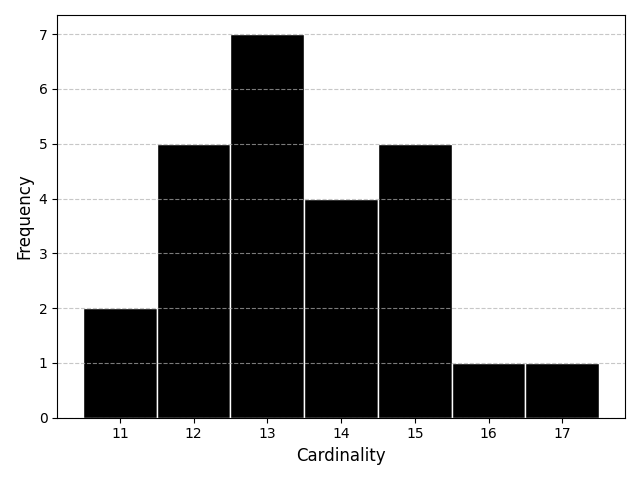
\includegraphics[width=\textwidth]{../figures/wine_cardinalities}
        \caption{Wine Dataset}
        \label{fig:wine_cardinalities}
    \end{subfigure}
    \hfill
    % Iris
    \begin{subfigure}[b]{0.45\textwidth}
        \centering
        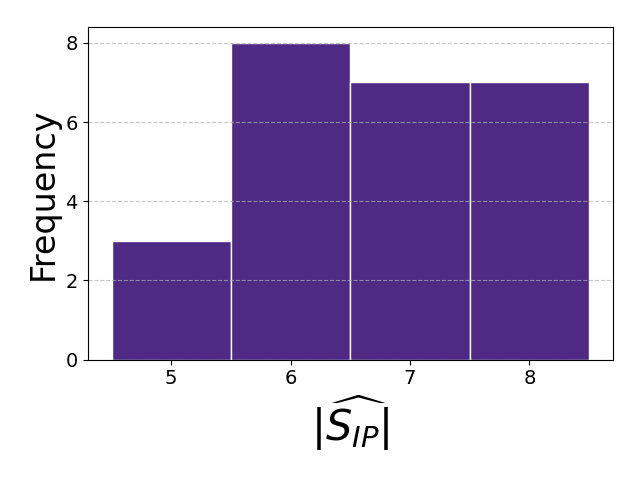
\includegraphics[width=\textwidth]{../figures/iris_cardinalities}
        \caption{Iris Dataset}
        \label{fig:iris_cardinalities}
    \end{subfigure}

    \vspace{0.5em}  % small vertical space between rows

    % Ethanol
    \begin{subfigure}[b]{0.45\textwidth}
        \centering
        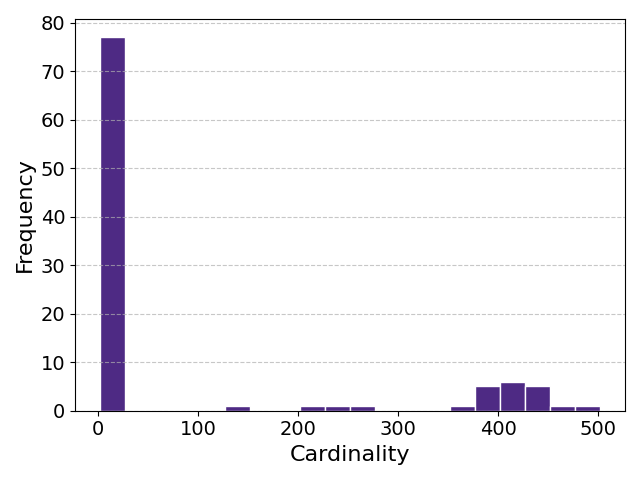
\includegraphics[width=\textwidth]{../figures/ethanol_cardinalities}
        \caption{Ethanol Dataset}
        \label{fig:ethanol_cardinalities}
    \end{subfigure}
    \hfill
    % Words
    \begin{subfigure}[b]{0.45\textwidth}
        \centering
        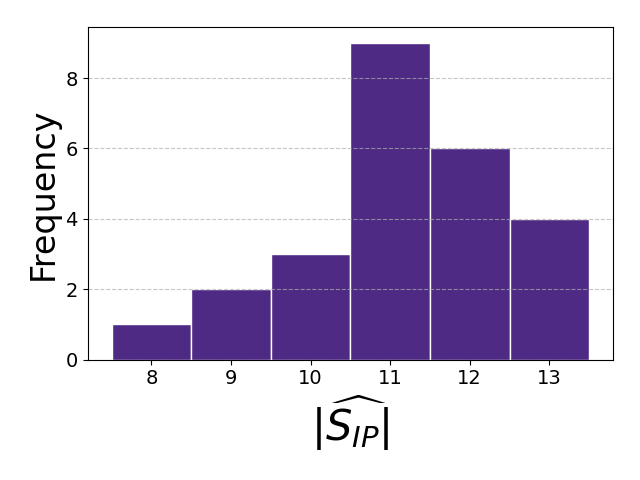
\includegraphics[width=\textwidth]{../figures/words_cardinalities}
        \caption{Words Dataset}
        \label{fig:words_cardinalities}
    \end{subfigure}

    \caption{Support cardinalities for each dataset under Basis Pursuit.}
    \label{fig:support_cardinalities}
\end{figure}


\newpage

\subsection{Proposition \ref{prop:unitary_selection} deep dive}
\label{sec:deep_dive}

The results in Section \ref{sec:experiments} show that there are circumstances in which the \greedy~ performs better than \tsip, so clearly \tsip~ does not always achieve a global optimum.
Figure \ref{fig:ecdf_comparison_losses} gives results on the line of inquiry about why this is the case based on the reasoning presented in Section \ref{sec:discussion}.
In these results a two-stage algorithm achieves the global optimum of a slightly different brute problem, namely brute optimization of the multitask basis pursuit penalty $\|\cdot \|_{1,2}$.
That is, brute search on $\|\cdot \|_{1,2}$ gives the same result as the two stage algorithm with brute search on $\|\cdot \|_{1,2}$ subsequent to isometry pursuit.
This suggests that failure to select the global optimum by \tsip~ is due to the mismatch between global optimums of brute optimization of the multitask penalty and the isometry loss given certain data.
It also confirms that the minimizer of brute optimization of the $\|\|_{1,2}$ objective is contained within the isometry pursuit solution.
Note that this would include an isometric solution, should it exist.

\begin{figure}[t]
    \centering
    % Top-left plot: Iris Isometry Loss ECDF
    \begin{subfigure}[b]{0.45\textwidth}
        \centering
        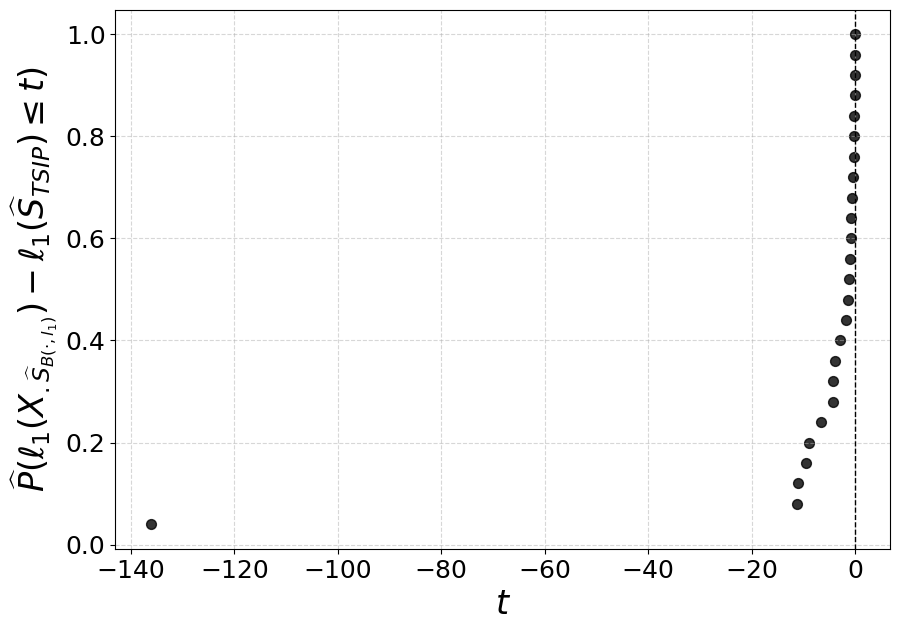
\includegraphics[width=\textwidth]{../figures/iris_isometry_losses_iso_ecdf}
        \caption{Iris $\ell_1(X_{.\widehat S})$ comparison for brute optimization of $\ell_1$ versus two-stage Isometry Pursuit optimization of $\ell_1$}
        \label{fig:iris_isometry_losses_ecdf}
    \end{subfigure}
    \hfill
    % Top-right plot: Iris Multitask Loss ECDF
    \begin{subfigure}[b]{0.45\textwidth}
        \centering
        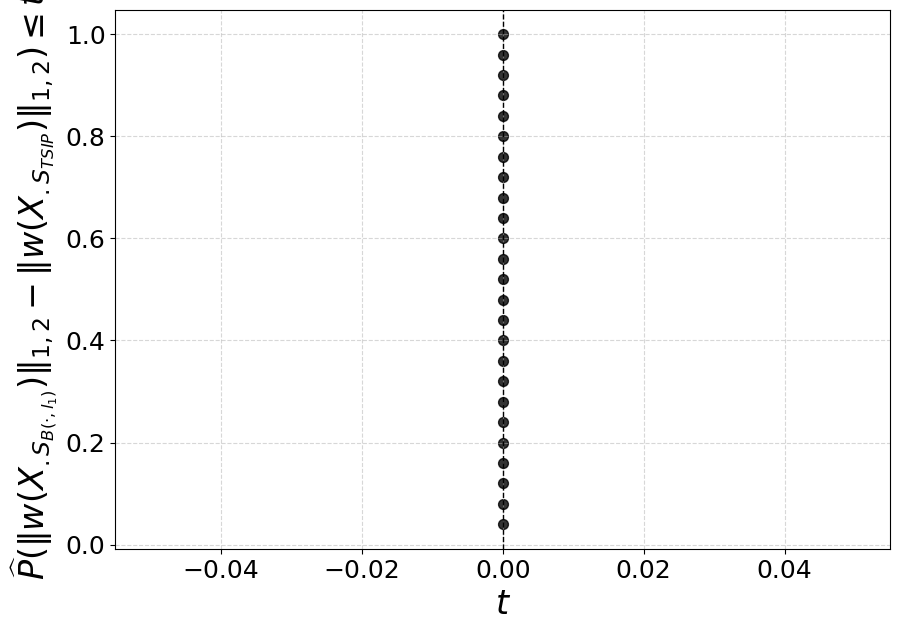
\includegraphics[width=\textwidth]{../figures/iris_isometry_losses_ts_ecdf}
        \caption{Iris $\|X_{.\widehat S}\|_{1,2}$ comparison for brute optimization of $\|\|_{1,2}$ versus two-stage Isometry Pursuit optimization of $\|\|_{1,2}$}
        \label{fig:iris_multitask_losses_ecdf}
    \end{subfigure}

    \vspace{0.5cm}

    % Bottom-left plot: Wine Isometry Loss ECDF
    \begin{subfigure}[b]{0.45\textwidth}
        \centering
        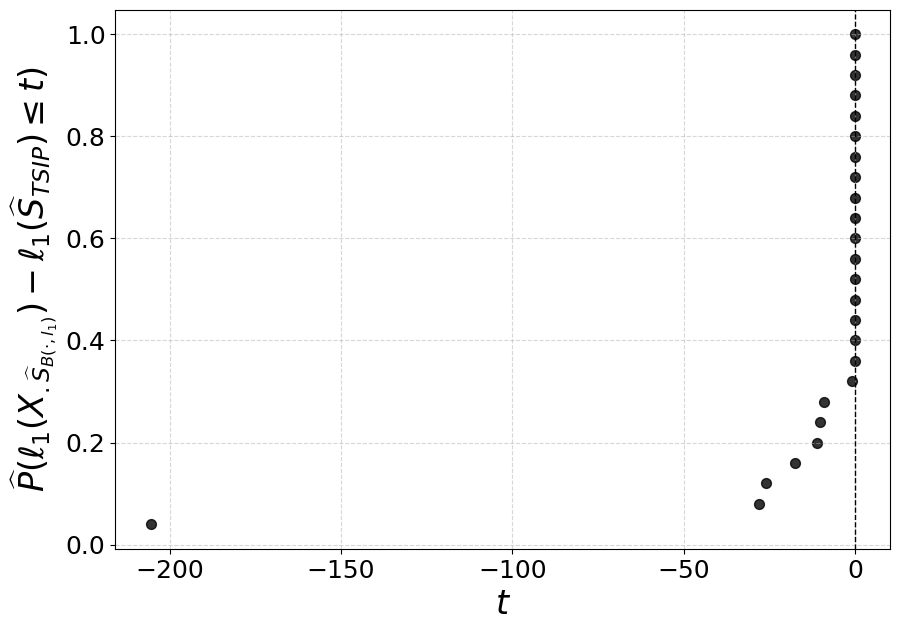
\includegraphics[width=\textwidth]{../figures/wine_isometry_losses_iso_ecdf}
        \caption{Wine $\ell_1(X_{.\widehat S})$ comparison for brute optimization of $\ell_1$ versus two-stage Isometry Pursuit optimization of $\ell_1$}
        \label{fig:wine_isometry_losses_ecdf}
    \end{subfigure}
    \hfill
    % Bottom-right plot: Wine Multitask Loss ECDF
    \begin{subfigure}[b]{0.45\textwidth}
        \centering
        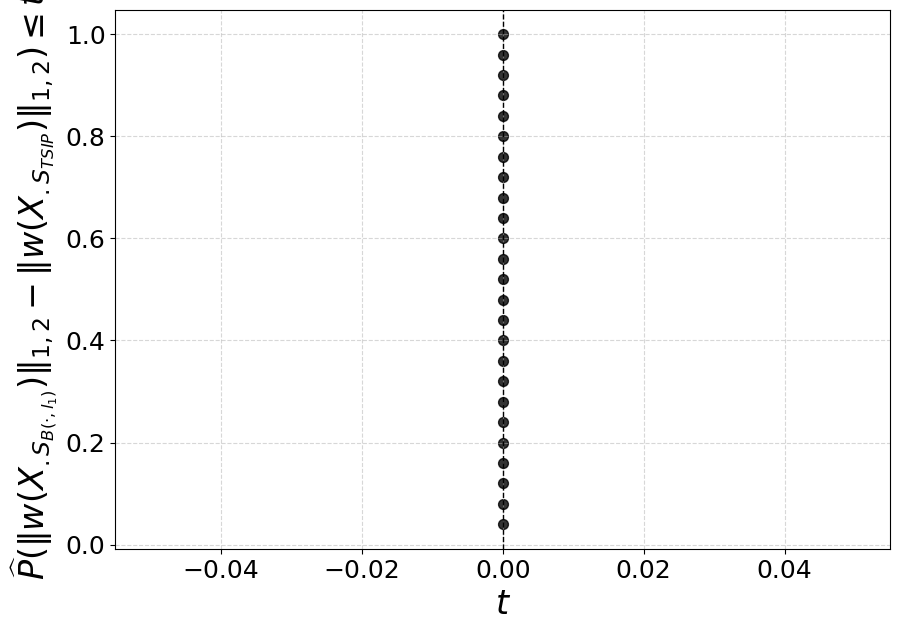
\includegraphics[width=\textwidth]{../figures/wine_isometry_losses_ts_ecdf}
        \caption{Wine $\|X_{.\widehat S}\|_{1,2}$ comparison for brute optimization of $\|\|_{1,2}$ versus two-stage Isometry Pursuit optimization of $\|\|_{1,2}$}
        \label{fig:wine_multitask_losses_ecdf}
    \end{subfigure}

    \caption{Comparison of Isometry and Group Lasso Losses across $25$ replicates for randomly downsampled Iris and Wine Datasets with $(P,D) = (4,15)$ and $(13, 18)$, respectively.
    Note that this further downsampling compared with Section \ref{sec:experiments} was necessary to compute global minimizers of \brute.
    Left column: isometry losses $\ell_1(X_{.\widehat{S}})$. Right column: multitask norms $\|w(X_{.\widehat{S}})\|_{1,2}$.
    }
    \label{fig:ecdf_comparison_losses}
\end{figure}

\newpage

\subsection{Word embeddings}
\label{sec:word_embeddings}

We applied \isometrypursuit~ on a word embedding dataset with the following construction.
We used all-MiniLM-L6-v2 from the Sentence Transformers library \citep{reimers-2019-sentence-bert}.
We defined $6$ axes of variation using the word categories shown in table \ref{tab:semantic_axes}
Each axis is defined by the difference between two poles, computed from the centroids of the embeddings of the corresponding word sets.
We then projected the word embeddings onto these axes and standardized in order to create a linear conceptual embedding space.
This was the representation that we evaluated.

\begin{table}[t]
\centering
\begin{tabular}{|c|c|c|p{5cm}|p{5cm}|}
\hline
\textbf{Pole 1} & \textbf{Pole 2} & \textbf{Category} & \textbf{Words (Pole 1)} & \textbf{Words (Pole 2)} \\
\hline
man     & woman     & gender   & man, male, guy, gentleman, sir & woman, female, lady, madam, gal \\
regent  & slave     & status   & regent, sovereign, monarch, emperor, pharaoh & slave, wench \\
young   & old       & age      & young, kid & old, elderly \\
warrior & scholar   & domain   & warrior, soldier, knight, fighter, mercenary & scholar, academic, professor, intellectual, scientist \\
rich    & poor      & wealth   & rich, wealthy, affluent, millionaire, tycoon & poor, impoverished, broke, destitute, beggar \\
urban   & rural     & location & urban, city, metropolitan, cosmopolitan, downtown & rural, village, countryside, agrarian, pastoral \\
warm    & cold      & warmth   & warm, friendly, kind, loving, affectionate & cold, aloof, harsh, distant, indifferent \\
\hline
\end{tabular}
\caption{Semantic axes used for projection of word embeddings. }
\label{tab:semantic_axes}
\end{table}

In order to illustrate the semantic interpretation of our analyses, we plot the following co-occurrence graph for retrieved words.
While we do not provide any additional quantitative evaluation, in the plotted replicate two-stage Isometry Pursuit better separates words from the same category (e.g. cold, warm) than does greedy search.

\begin{figure}[h]
    \centering
    % First graph
    \begin{subfigure}[b]{0.47\textwidth}
        \centering
        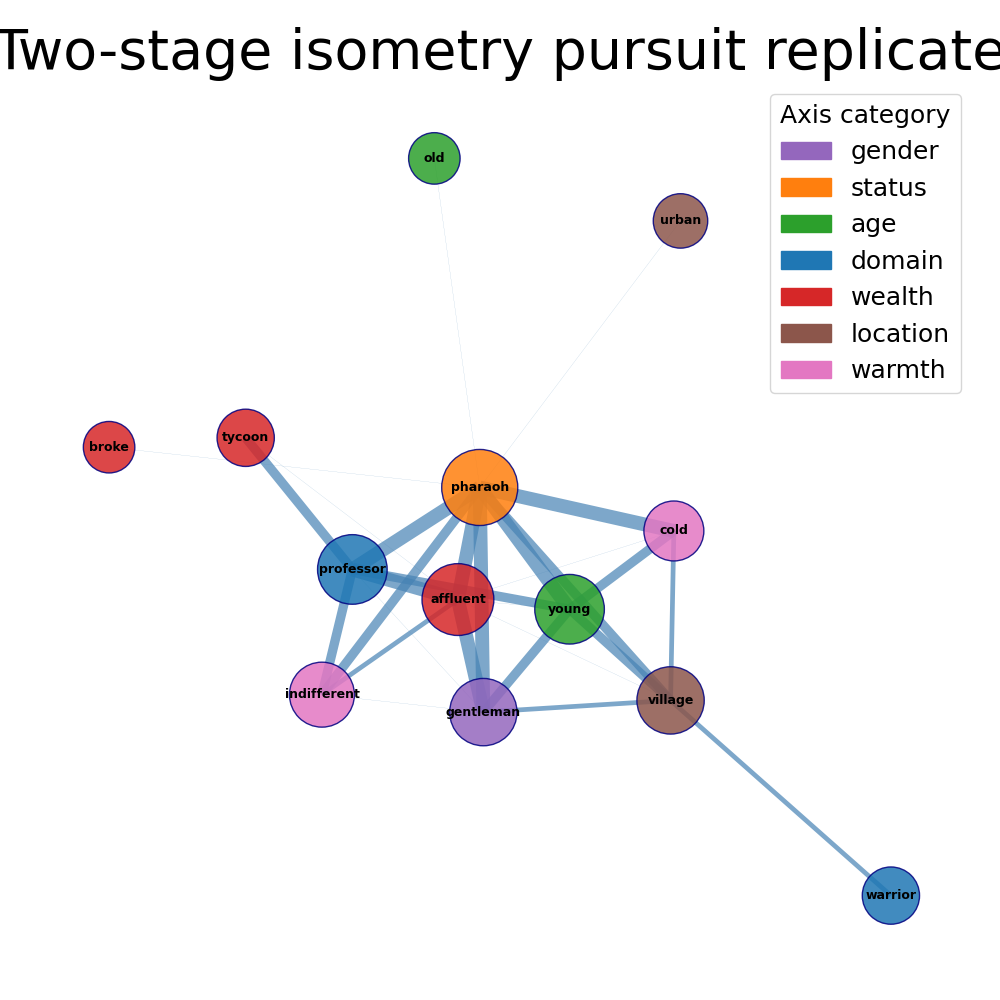
\includegraphics[width=\textwidth]{../figures/ip_graph.png}
        \caption{Two-stage isometry pursuit selected word co-occurrences}
        \label{fig:co_occurrence_brute}
    \end{subfigure}
    \hfill
    % Second graph
    \begin{subfigure}[b]{0.47\textwidth}
        \centering
        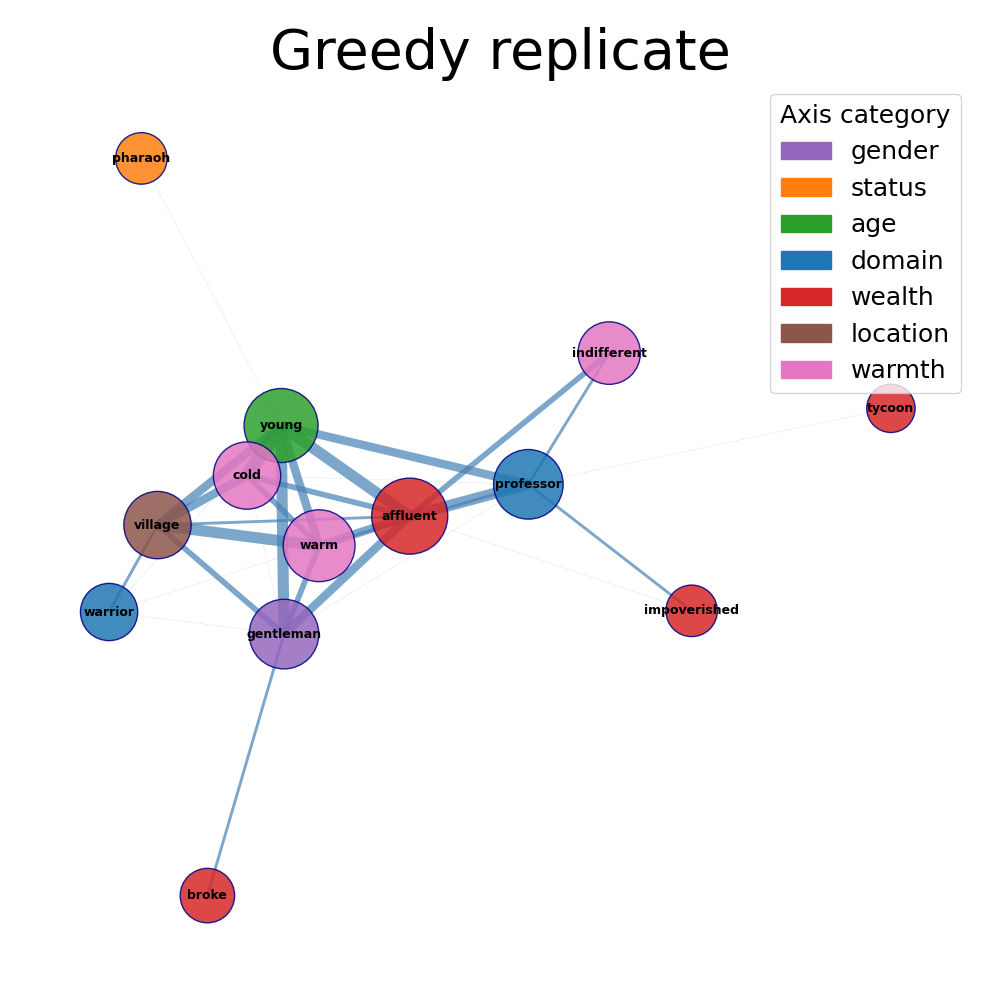
\includegraphics[width=\textwidth]{../figures/greedy_graph.png}
        \caption{Greedy algorithm selected word co-occurrences}
        \label{fig:co_occurrence_two_stage}
    \end{subfigure}
    
    \caption{Force-directed graphs of word co-occurrences for each selection method.
    Node size reflects marginal frequency across replicates.
    Edge width represents co-occurrence strength ($\geq 5$).
    Colors denote semantic axis.}
    \label{fig:co_occurrence_graphs}
\end{figure}




\subsection{Timing}
\label{sec:timing}

While wall-time of algorithms is a non-theoretical quantity that depends on implementation details, it provides valuable context for practitioners.
We therefore report the following runtimes on a 2021 Macbook Pro.
The particularly high variance for brute force search in the second step of \tsip~ is likely due to the large cardinalities reported in Figure \ref{fig:support_cardinalities}.

\begin{table}[H]
\centering
\begin{tabular}{|c|c|c|c}
\toprule
Name & IP & 2nd stage & Greedy \\
\midrule
Iris & 1.24 ± 0.02 & 0.00 ± 0.00 & 0.02 ± 0.00 \\
Wine & 2.32 ± 0.17 & 0.13 ± 0.12 & 0.03 ± 0.00 \\
Ethanol & 8.38 ± 0.57 & 0.55 ± 1.08 & 0.07 ± 0.01 \\
Words & 0.98 ± 0.20 & 0.03 ± 0.02 & 0.01 ± 0.00 \\
\bottomrule
\end{tabular}
\caption{Algorithm runtimes in seconds across replicates.}
\end{table}